% Itt kezdődik a dolgozat lényegi része, úgy értve, hogy a saját munka bemutatása.
% Jellemzően ebben szerepelni szoktak blokkdiagramok, a program struktúrájával foglalkozó leírások.
% Ehhez célszerű UML ábrákat (például osztály- és szekvenciadiagramokat) használni.

% Amennyiben a dolgozat inkább kutatás jellegű, úgy itt lehet konkretizálni a kutatási módszertant, a kutatás tervezett lépéseit, az indoklást, hogy mit, miért és miért pont úgy érdemes csinálni, ahogyan az a későbbiekben majd részletezésre kerül.

% Ebben a fejezetben az implementáció nem kell, hogy túl nagy szerepet kapjon.
% Ez még csak a tervezési fázis.
% (Nyilván ha olyan a téma, hogy magának az implementációnak a módjával foglalkozik, adott formális nyelvet mutat be, úgy a kódpéldákat már innen sem lehet kihagyni.)

% \Section{Táblázatok}

% Táblázatokhoz a \texttt{table} környezetet ajánlott használni.
% Erre egy minta \aref{tab:minta}. táblázat.
% A hivatkozáshoz az egyedi \texttt{label} értéke konvenció szerint \texttt{tab:} prefixszel kezdődik.

% \begin{table}[h]
% \centering
% \caption{Minta táblázat. A táblázat felirata a táblázat felett kell legyen!}
% \label{tab:minta}
% \begin{tabular}{l|c|c|}
% a & b & c \\
% \hline
% 1 & 2 & 3 \\
% 4 & 5 & 6 \\
% \hline
% \end{tabular}
% \end{table}

% \Section{Ábrák}

% Ábrákat a \texttt{figure} környezettel lehet használni.
% A használatára egy példa \aref{fig:cimer}. ábrán látható.
% Az \texttt{includegraphics} parancsba 
% Az ábrák felirata az ábra alatt kell legyen.
% Az ábrák hivatkozásához használt nevet konvenció szerint \texttt{fig:}-el célszerű kezdeni.

% \begin{figure}[h]
% \centering
% 
\includegraphics[scale=0.3]{images/me_logo.png}
% \caption{A Miskolci Egyetem címere.}
% \label{fig:cimer}
% \end{figure}

% \Section{További környezetek}

% A matematikai témájú dolgozatokban szükség lehet tételek és bizonyításaik megadására.
% Ehhez szintén vannak készen elérhető környezetek.

% \begin{definition}
% Ez egy definíció
% \end{definition}

% \begin{lemma}
% Ez egy lemma
% \end{lemma}

% \begin{theorem}
% Ez egy tétel
% \end{theorem}

% \begin{proof}
% Ez egy bizonyítás
% \end{proof}

% \begin{corollary}
% Ez egy tétel
% \end{corollary}

% \begin{remark}
% Ez egy megjegyzés
% \end{remark}

% \begin{example}
% Ez egy példa
% \end{example}

\colorlet{punct}{red!60!black}
\definecolor{background}{HTML}{EEEEEE}
\definecolor{delim}{RGB}{20,105,176}
\colorlet{numb}{magenta!60!black}

\Chapter{Tervezés}

% TODO: Érdemes lenne részletezni magát az adatmodellt is, tehát hogy egy felhasználóhoz, feladathoz mik tartoznak. (Lehet a felületi tervek előtt vagy után is, szokták így-is úgy-is.)

\Section{Kinézet}
A kinézetet játékos, egyszerű és átláthatóra szeretném csinálni, valamint mindenhol játékos ikonokat és színvilágot szeretnék használni. Az oldal ikonja az alábbi lett mivel minden teszt egy Game Boy-ként fog megjelenni:

\begin{figure}[h]
    \centering
    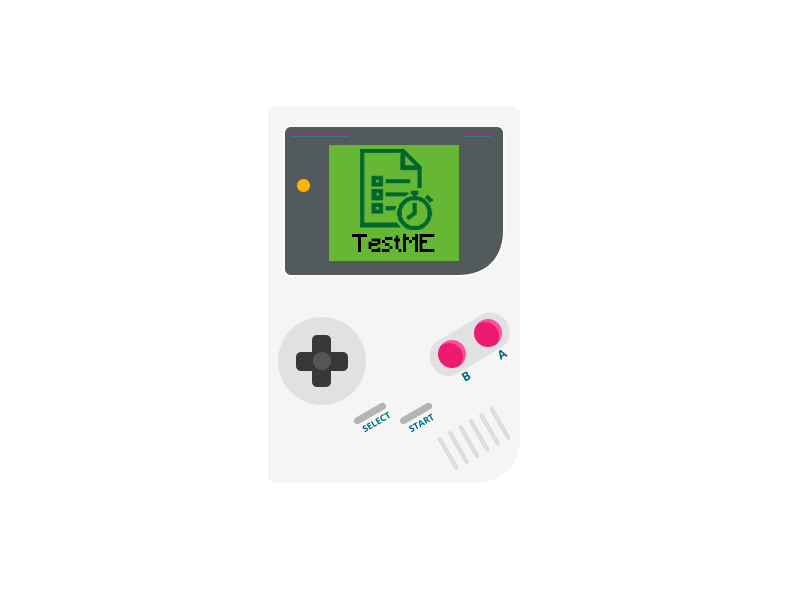
\includegraphics[height=5cm]{images/gameboy.png}
\end{figure}


Minden grafikus elemnél szeretném ha egységes lenne, így törekszem arra hogy hasonló stílusú legyen minden. Az egyéb funkciókhoz vagy oldalakhoz társított ikonok is élénkek, színesek, egyszerűek és vidámak lesznek hogy passzoljon az oldalhoz.

Az ikonokat a Flaticon nevű oldalról töltöttem le \cite{falcon}.
% TODO: Leírni, hogy az ikonok honnan származnak.

Valamint Bootstrap-et szeretnék használni ami egy olyan keretrendszer, amely segít a weboldalak gyorsabb és könnyebb megtervezésében. HTML és CSS alapú tervezősablonokat tartalmaz a tipográfiához, űrlapokat, gombokat, táblázatokat, navigációt, modelleket stb. Ez segítene abban hogy az oldalon egységes kinézetet hozhassak létre valamit a Bootstrap CSS-je alkalmazkodik a telefonokhoz, táblagépekhez és asztali számítógépekhez is.

\Section{Az oldal felépítése}

A funkciók elrendezésének és felépítésének bemutatására képernyőterv vázlatot (magyarul drótváznak, angolul wireframe vagy mockup-nak is nevezzük) készítettem a MockFlow \ref{mockflow} nevű oldalon.
Először azt az oldalt mutatom be amivel mindenki először találkozik az oldal megnyitásakor, ez pedig a bejelentkezési és regisztrációs felület.

\subsection{Bejelentkezés és regisztráció}

\begin{figure}[H]
    \centering
    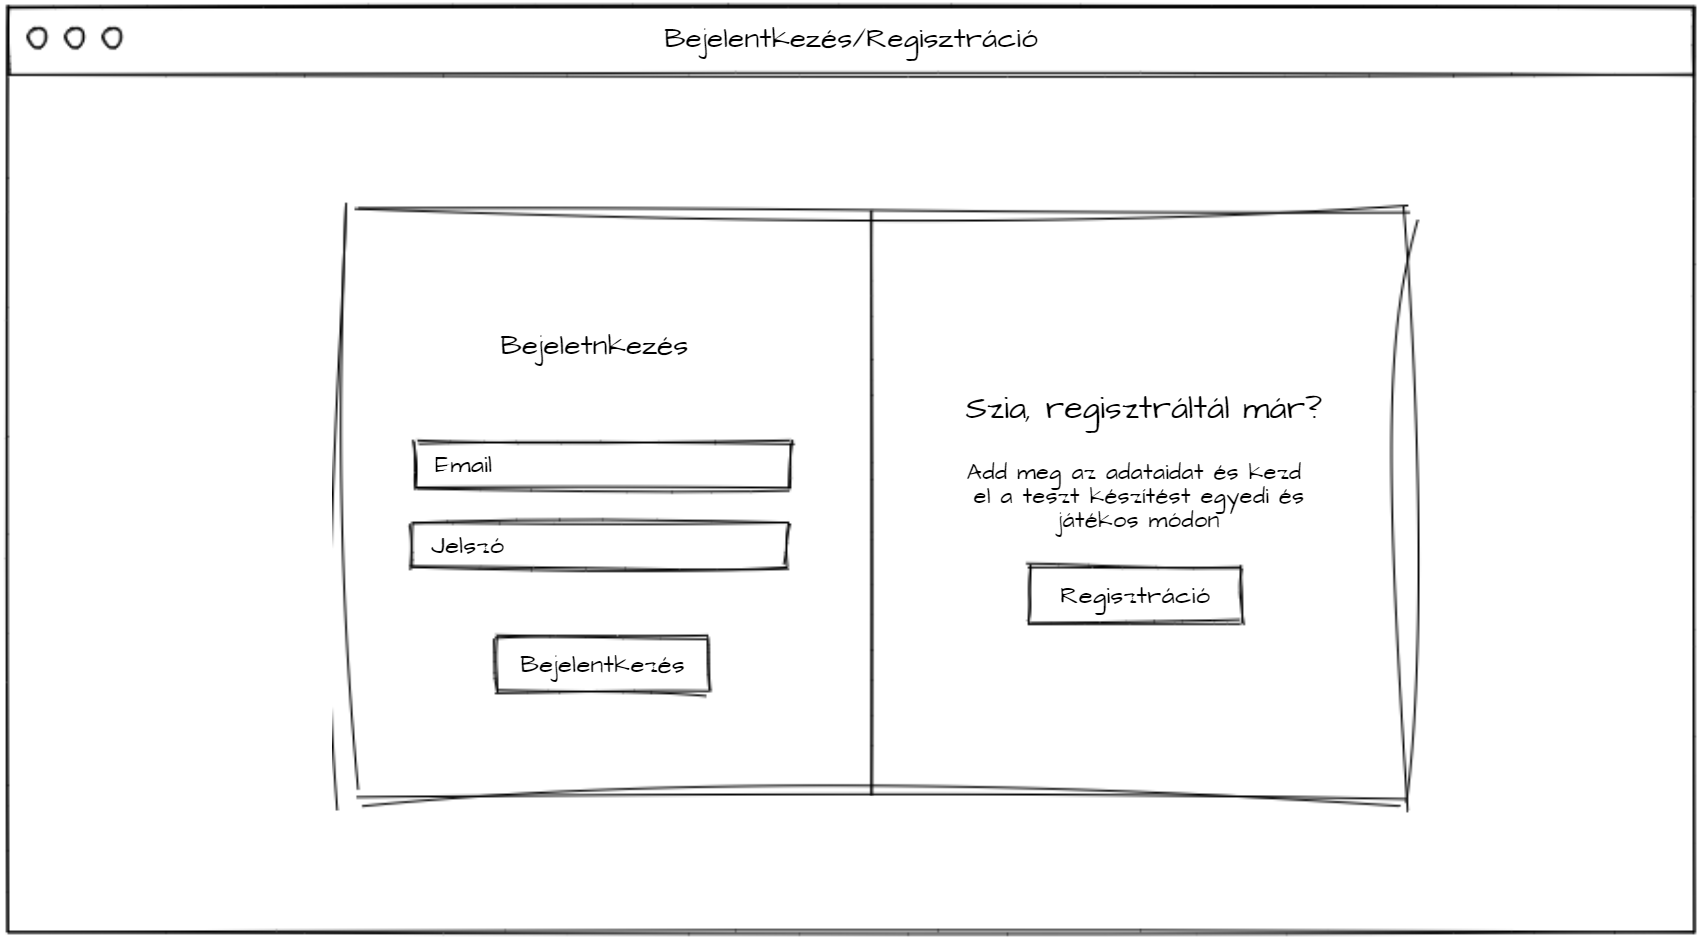
\includegraphics[width=\linewidth]{images/login_wireframe.png}
    \caption{Bejelentkezés}
    \label{fig:login_wireframe}
\end{figure}

\begin{figure}[H]
    \centering
    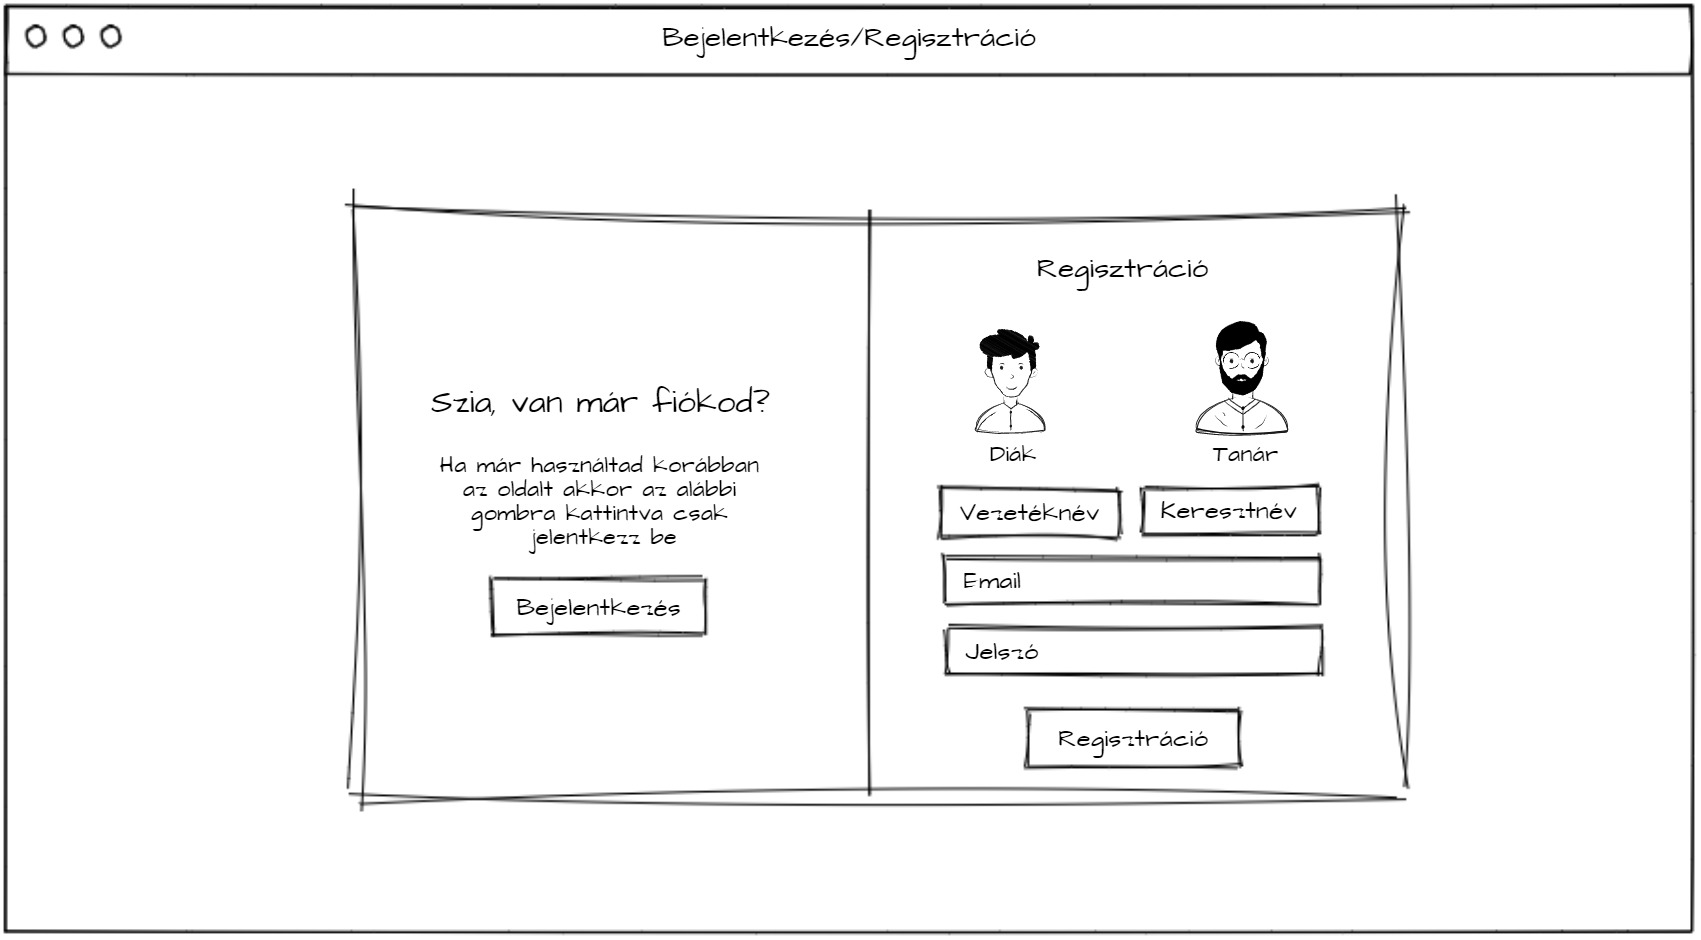
\includegraphics[width=\linewidth]{images/signin_wireframe.png}
    \caption{Regisztráció}
    \label{fig:signin_wireframe}
\end{figure}

Bejelentkezni \prettyref{fig:login_wireframe} email cím és jelszóval lehet. Regisztrációkor \prettyref{fig:signin_wireframe} pedig ki kell választani, hogy tanár vagy diákként szeretnénk regisztrálni majd meg kell adni az alapvető adatokat.
Ezután ha sikeresen beléptünk vagy regisztráltunk akkor hozzáférhetünk az oldalhoz.

\subsection{Főoldal}

\begin{figure}[H]
    \centering
    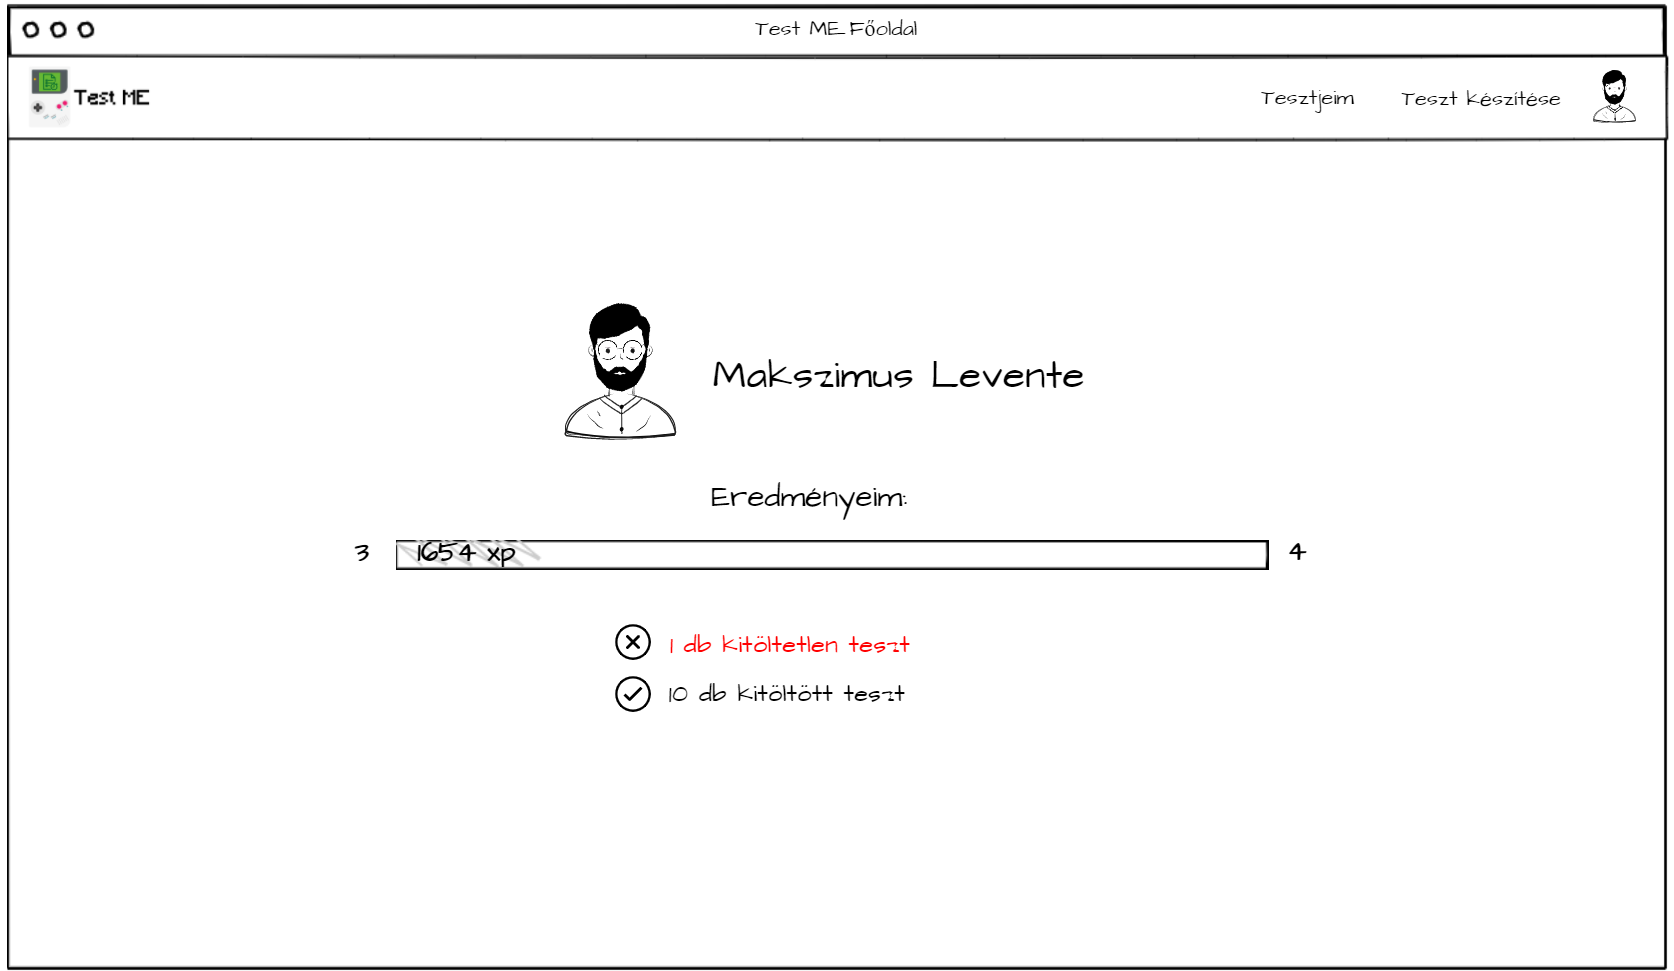
\includegraphics[width=\linewidth]{images/main_login_wireframe.png}
    \caption{Főoldal}
    \label{fig:main_page}
\end{figure}

Itt láthatjuk \prettyref{fig:main_page} a felhasználónevünket, hogy mennyi xp-vel rendelkezünk, hányas szintűek vagyunk és hogy hány darab kitöltött és kitöltetlen tesztünk van még.

\subsection{Teszt készítés}

\begin{figure}[H]
    \centering
    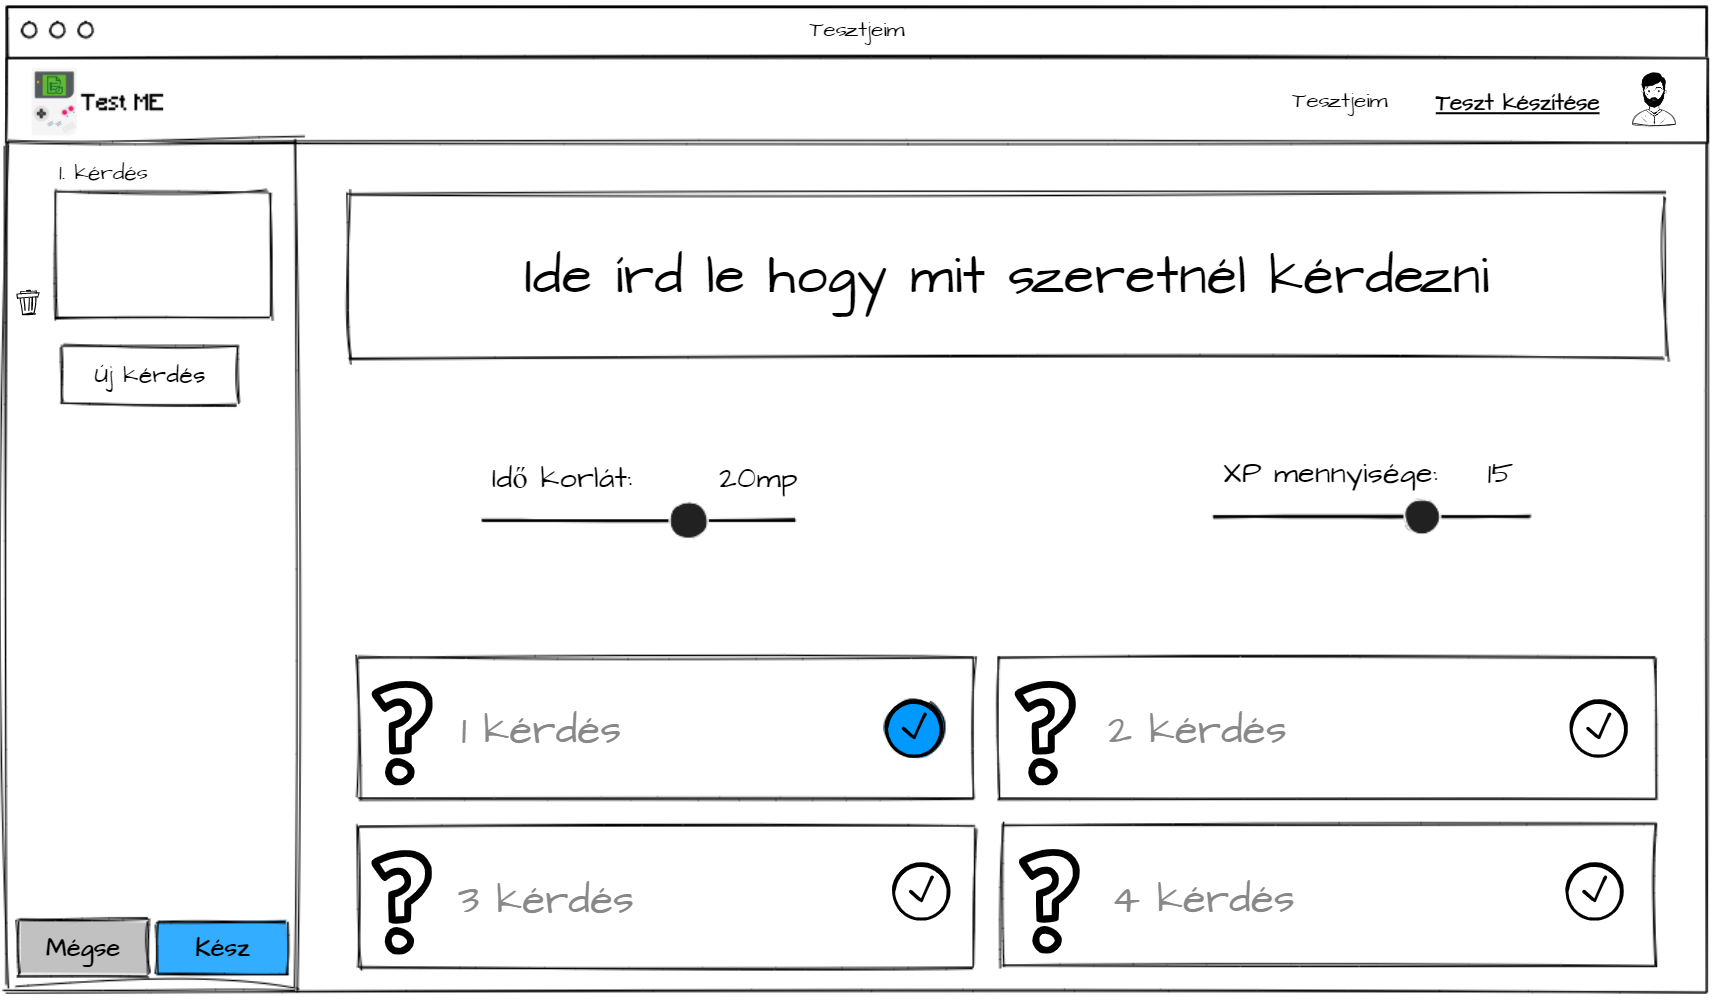
\includegraphics[width=\linewidth]{images/make_test_wireframe.png}
    \caption{Kvíz teszt készítés}
    \label{fig:new_quiz_question}
\end{figure}

Ezen a képen \prettyref{fig:new_quiz_question} a tesztkészítési felület látható. Egy tesztnél meghatározható maga a kérdés, ideje, illetve a jutalmazása, mely xp-ként van rögzítve. A választ kiválaszthatjuk az általunk írtak közül és beállíthatjuk melyik legyen a helyes megoldás.

\begin{figure}[H]
    \centering
    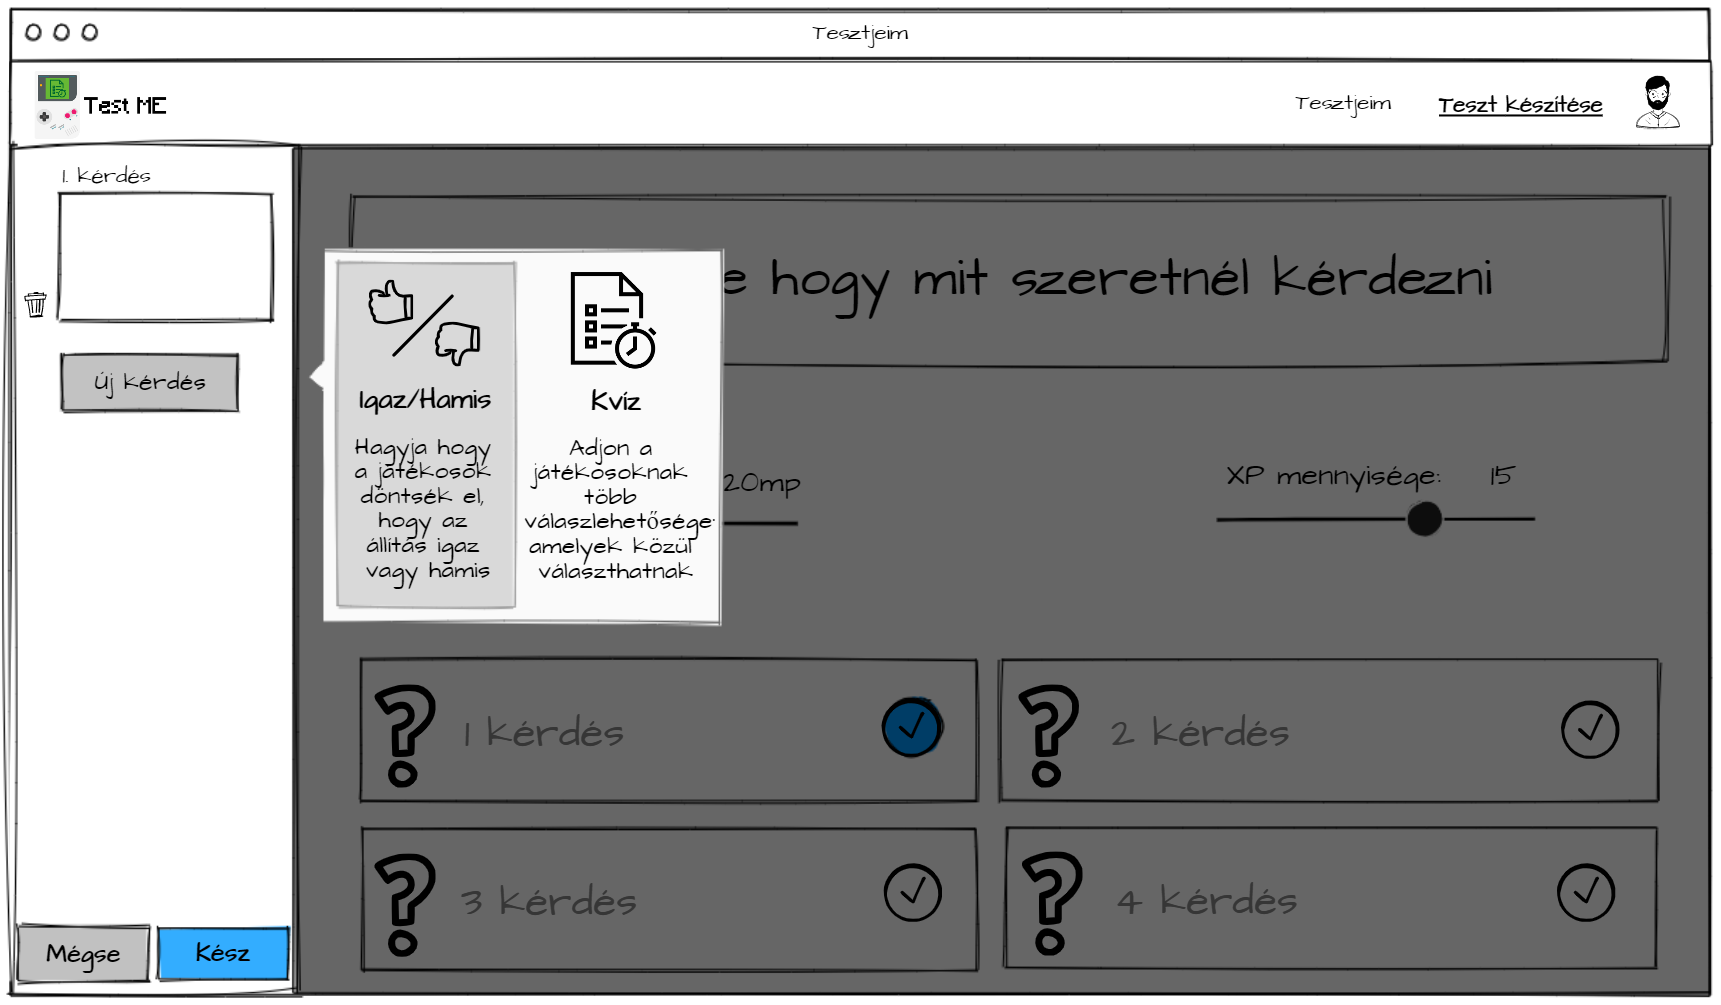
\includegraphics[width=\linewidth]{images/make_test2_wireframe.png}
    \caption{Új kérdés hozzáadása}
    \label{fig:new_question}
\end{figure}

Ezután ha elkészült a kérdés az "Új kérdés" gomb megnyomásával lehet hozzáadni a kérdések sorába. Itt választhatunk igaz/hamis, vagy kvíz típusú alternatíva közül, hogy milyet szeretnénk feltenni \prettyref{fig:new_question}.

\begin{figure}[H]
    \centering
    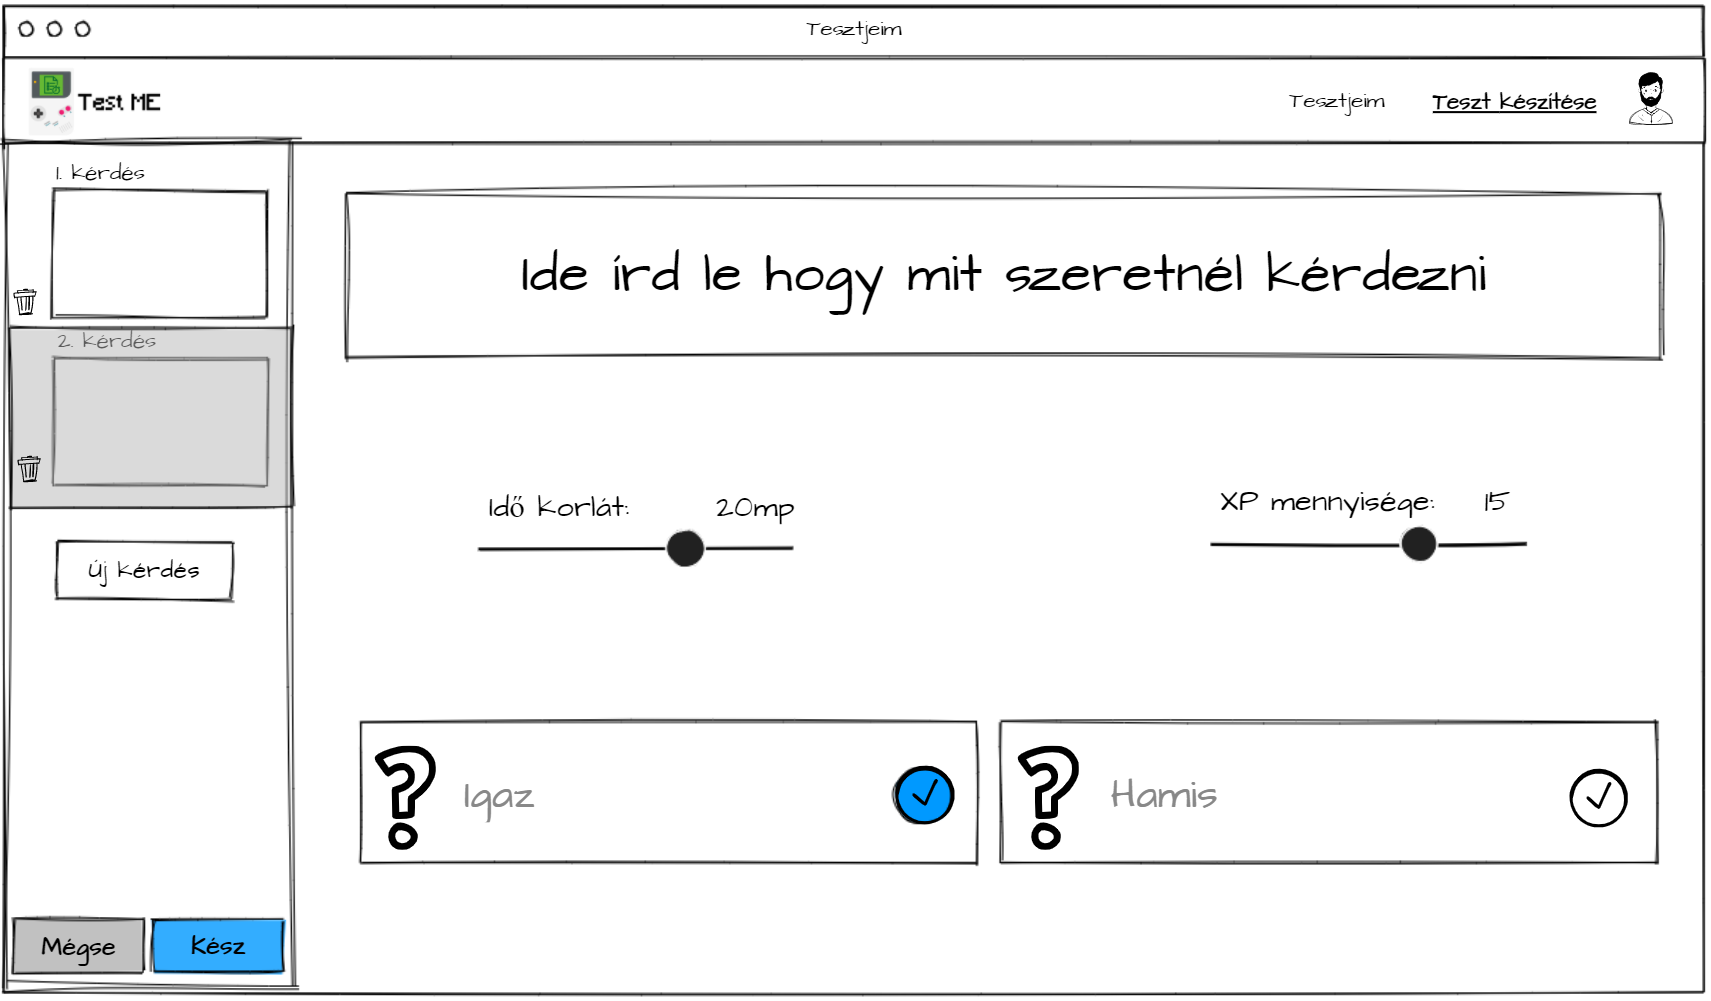
\includegraphics[width=\linewidth]{images/make_test3_wireframe.png}
    \caption{Igaz/hamis teszt készítése}
    \label{fig:test_true_false}
\end{figure}

Az igaz/hamis típusú kérdésnél csak annyi változik hogy nem lehet válasz lehetőséget írni, csak egy állítást amiről el kell dönteni, hogy valótlan vagy sem \prettyref{fig:test_true_false}.

\begin{figure}[H]
    \centering
    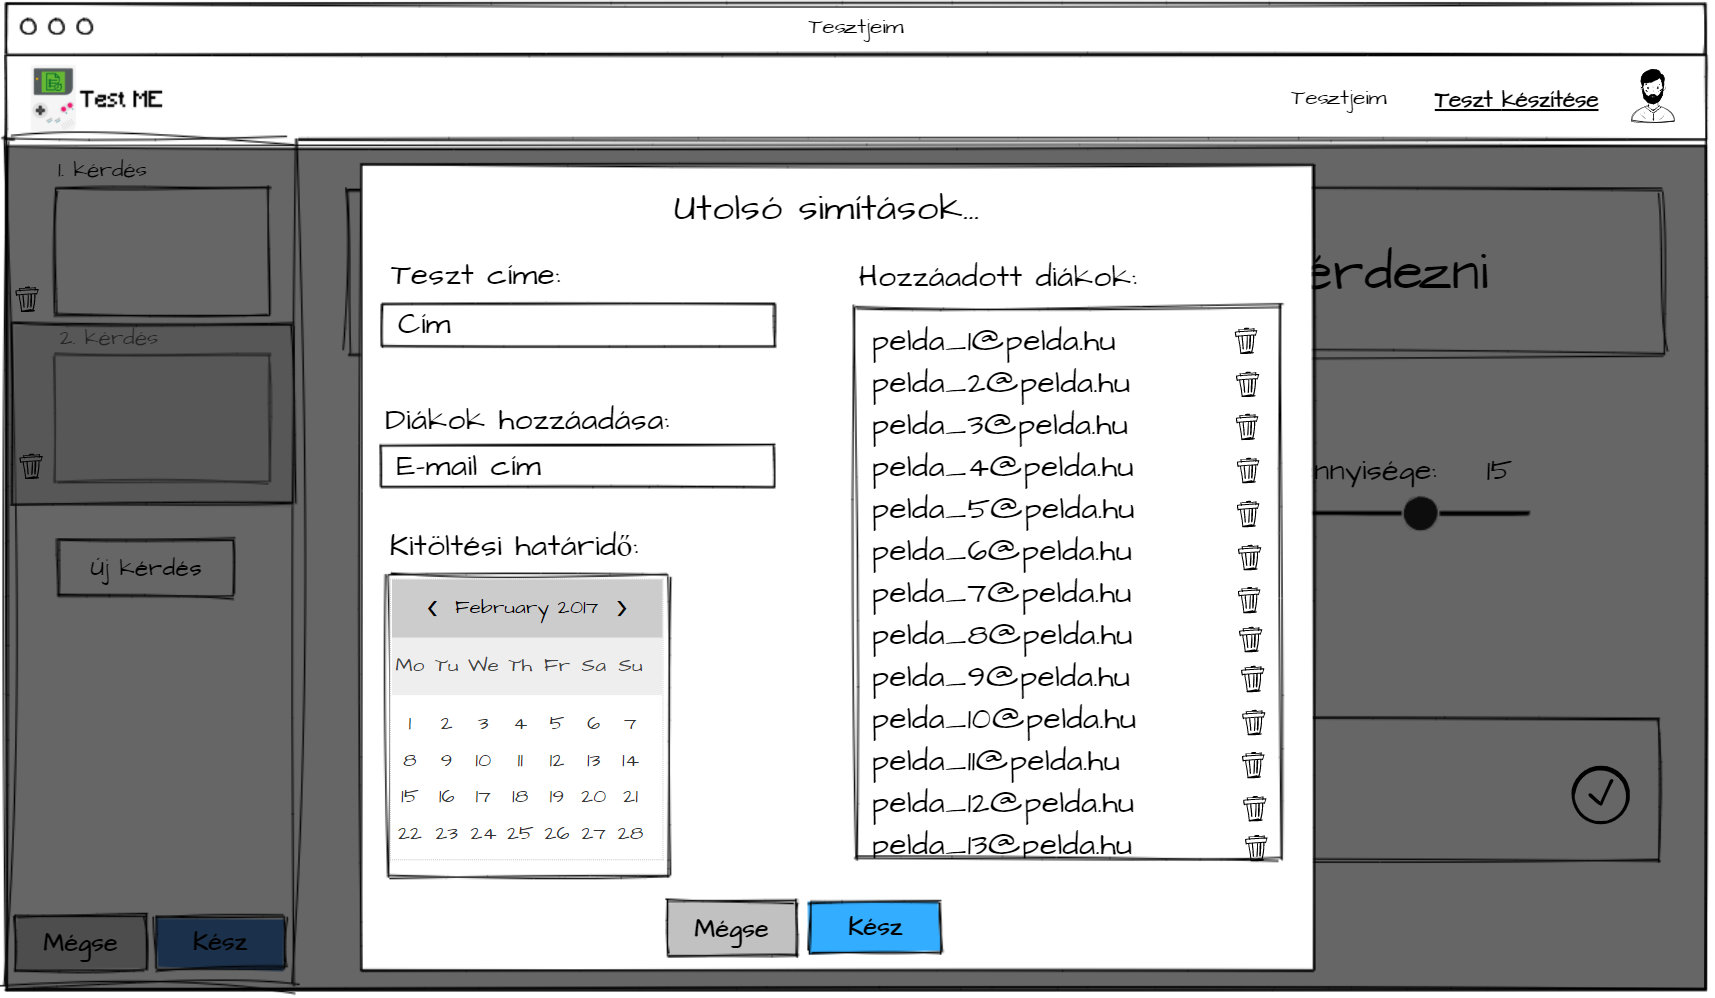
\includegraphics[width=\linewidth]{images/make_test4_wireframe.png}
    \caption{Adatok megadása és teszt elmentése}
    \label{fig:save_test}
\end{figure}

Az utolsó lépés pedig az hogy adunk címet a tesztnek, ilyen névvel fog megjelenni majd a diákoknak. Ezután hozzáadunk tetszőleges számú diákot akiktől szeretnénk hogy töltsék ki majd, egy kitöltési határidőt, és elkészült a tesztünk \prettyref{fig:save_test}.

\subsection{Saját tesztek}
\begin{figure}[H]
    \centering
    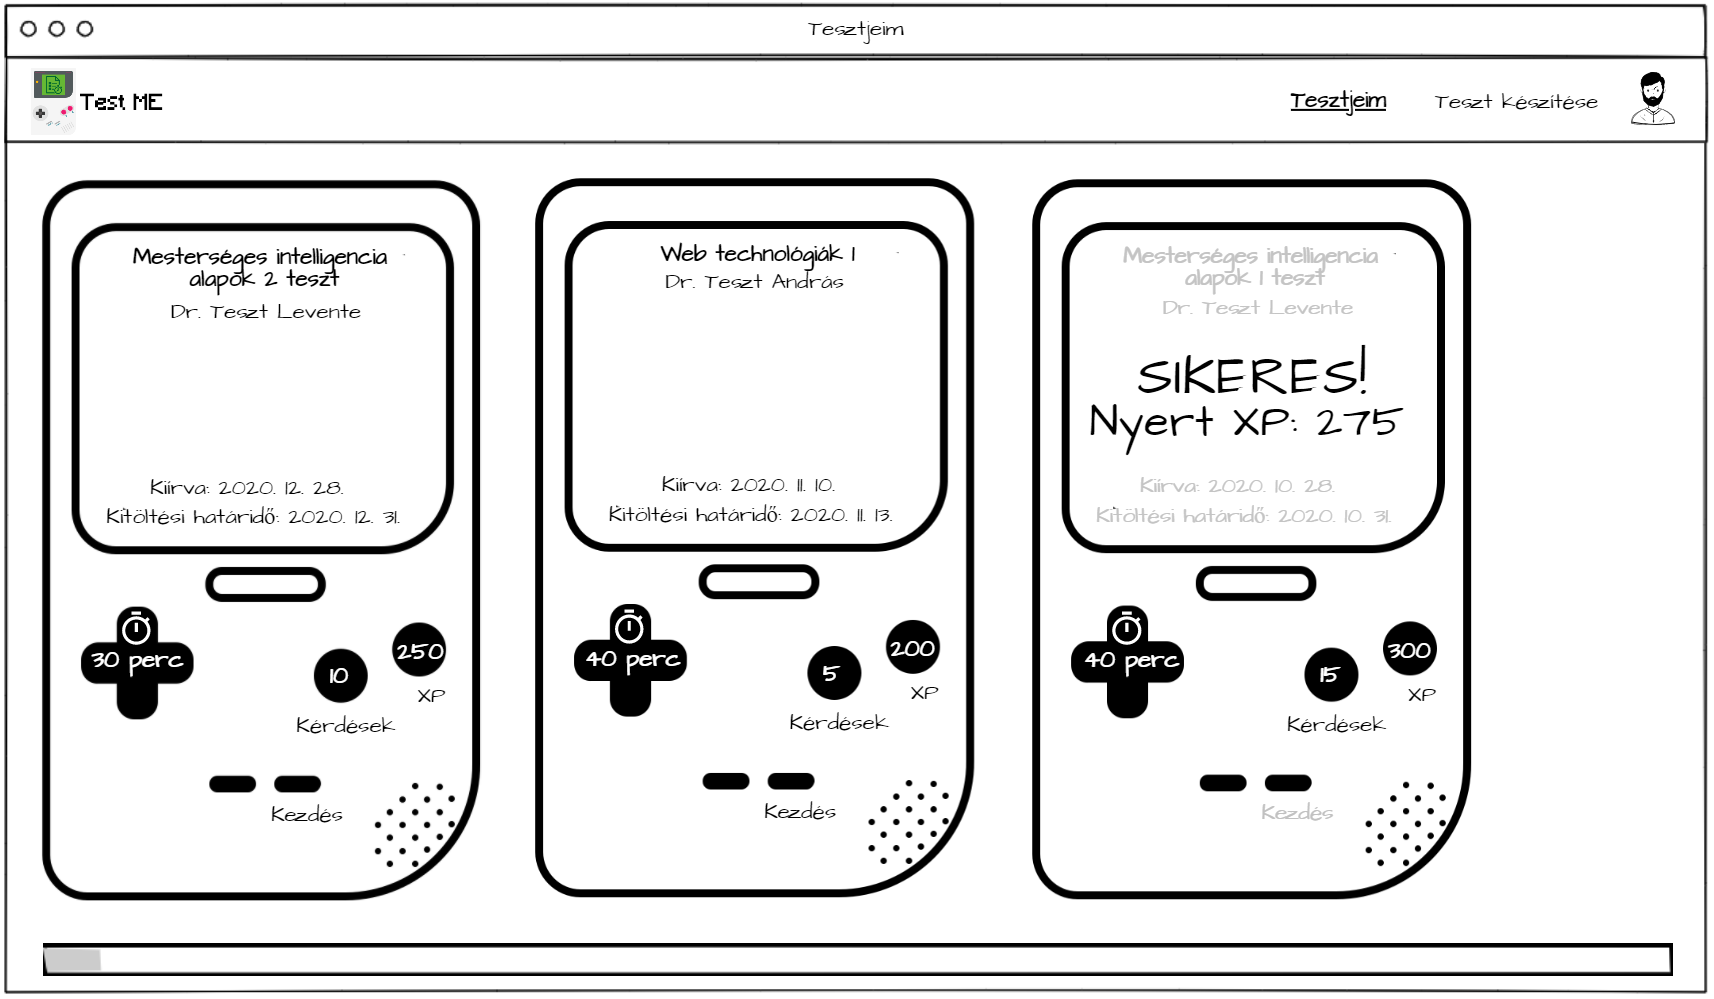
\includegraphics[width=\linewidth]{images/my_tests_wireframe.png}
    \caption{Felhasználóhoz rendelt tesztek}
    \label{fig:my_tests}
\end{figure}

Ezen a képen \prettyref{fig:my_tests} a diákhoz rendelt teszteket látjuk. Itt azok az adatok láthatóak amiket tesztkészítéskor adtunk meg. Tehát a kitöltési határidő, a teszt címe, mennyi idő van rá, hány kérdés van és hogy mennyi pontot lehet szerezni. Ezenkívül láthatjuk még hogy mikor lett kiírva és egy kezdés gombot amivel kitölthetjük.

\subsection{Teszt kitöltése}

\begin{figure}[H]
    \centering
    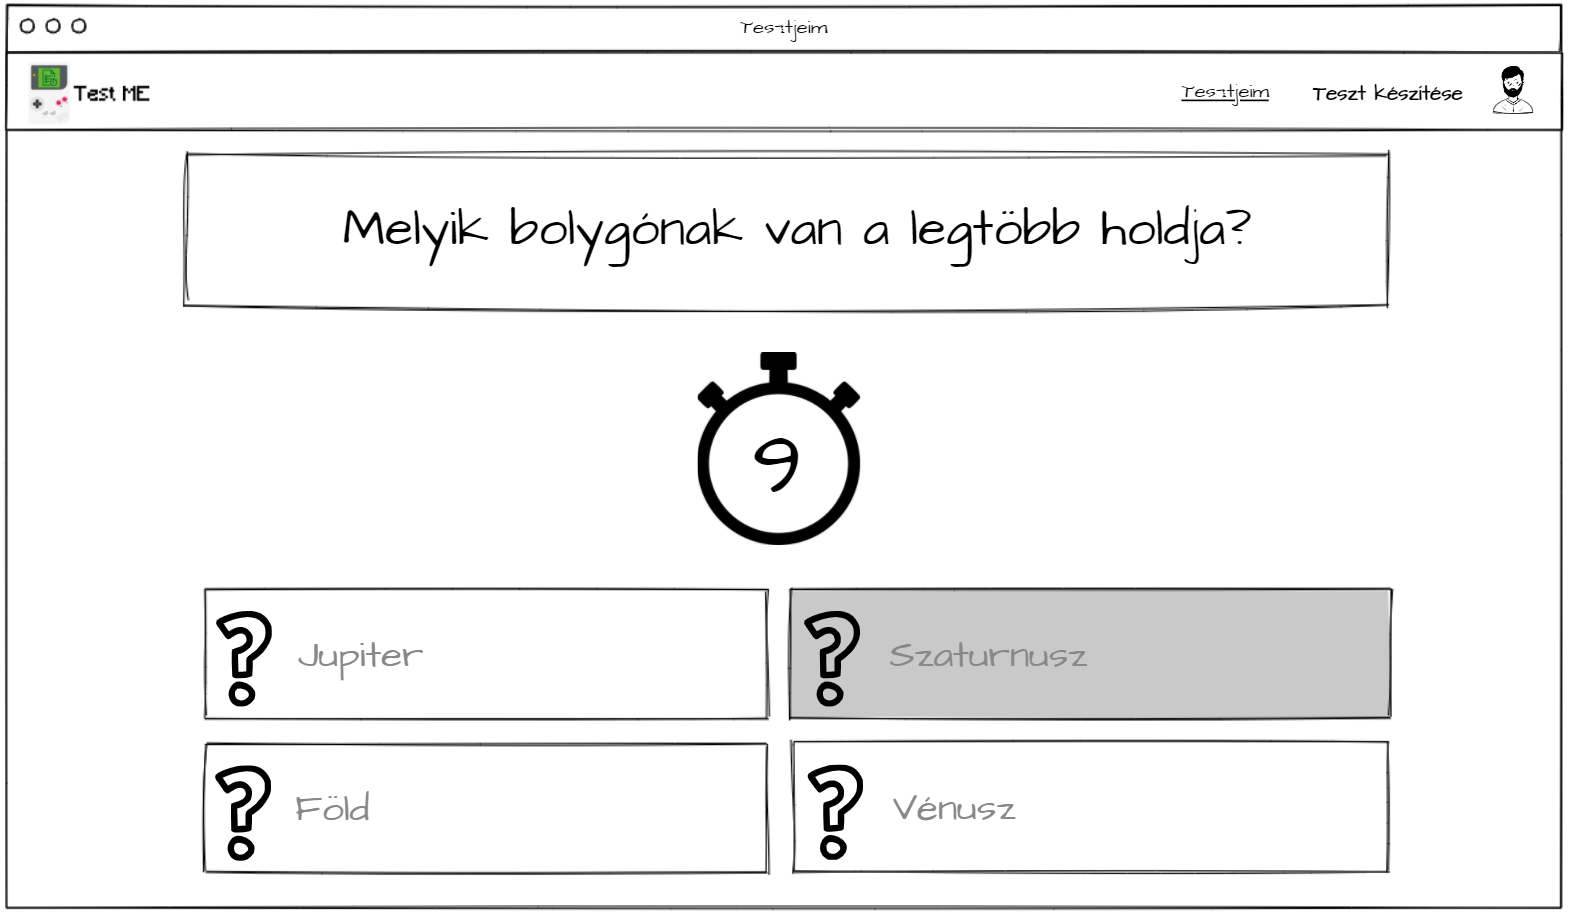
\includegraphics[width=\linewidth]{images/test1_wireframe.png}
    \caption{Feltett kérdés}
    \label{fig:test_question}
\end{figure}

Itt \prettyref{fig:test_question} egy kérdést látható teszt indítás után. Minden kérdésnél egy stopper órában láthatjuk hány másodpercünk van még válaszolni.

\begin{figure}[H]
    \centering
    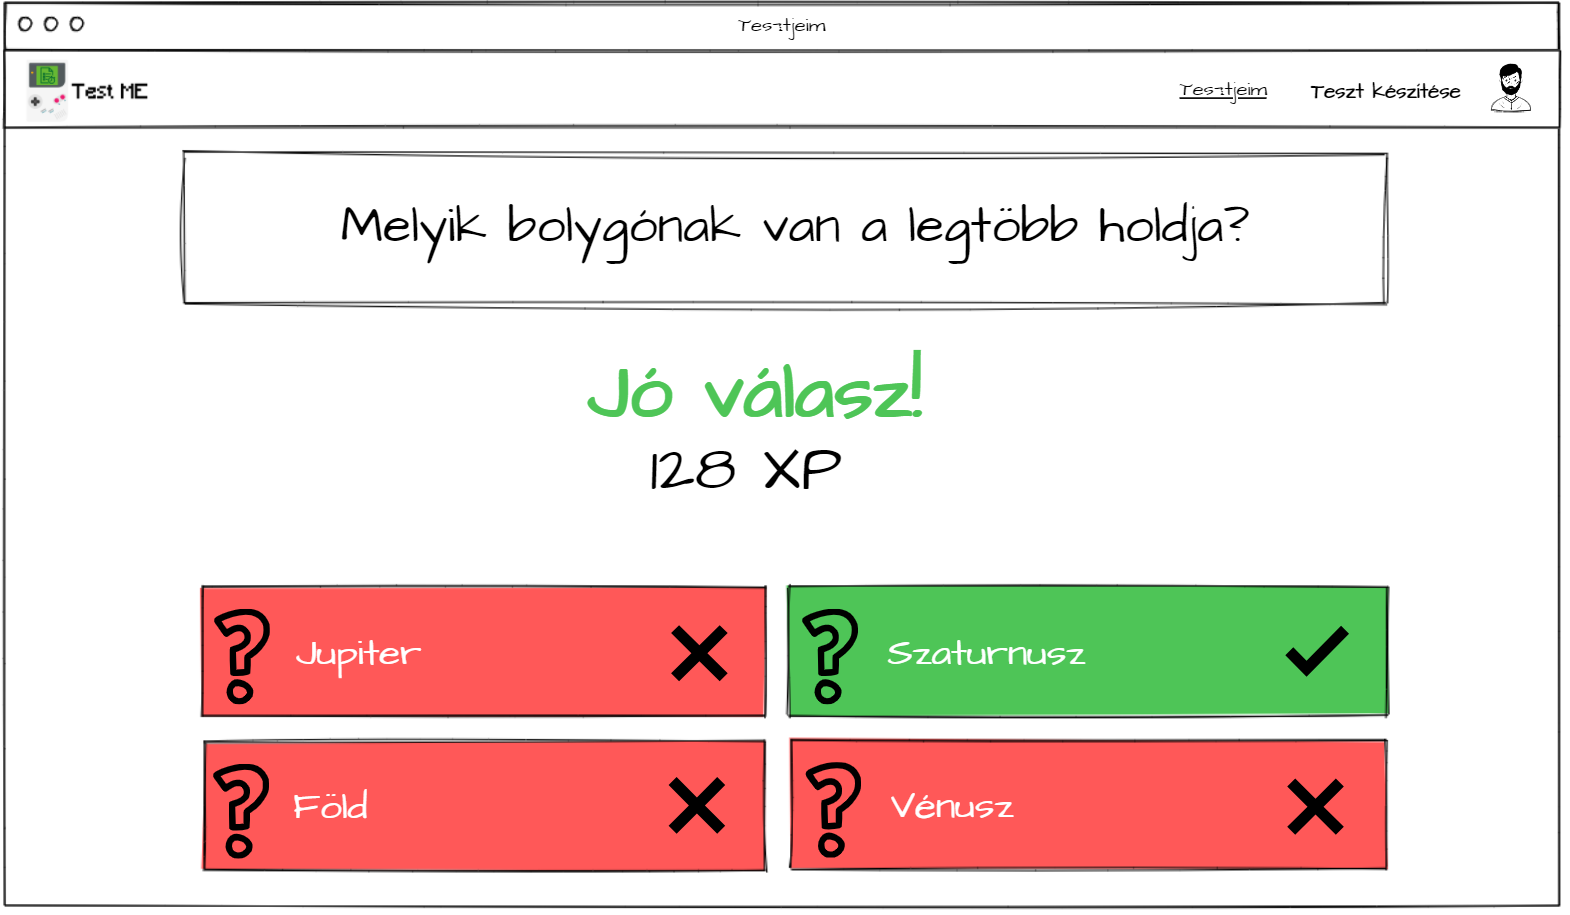
\includegraphics[width=\linewidth]{images/test2_wireframe.png}
    \caption{Válasz a kérdésre}
    \label{fig:test_answer}
\end{figure}

Válasz adás után pedig láthatjuk \prettyref{fig:test_answer} hogy ha válaszolunk egy kérdésre akkor melyik volt a jó és hogy válaszunk rossz vagy jó.

\begin{figure}[H]
    \centering
    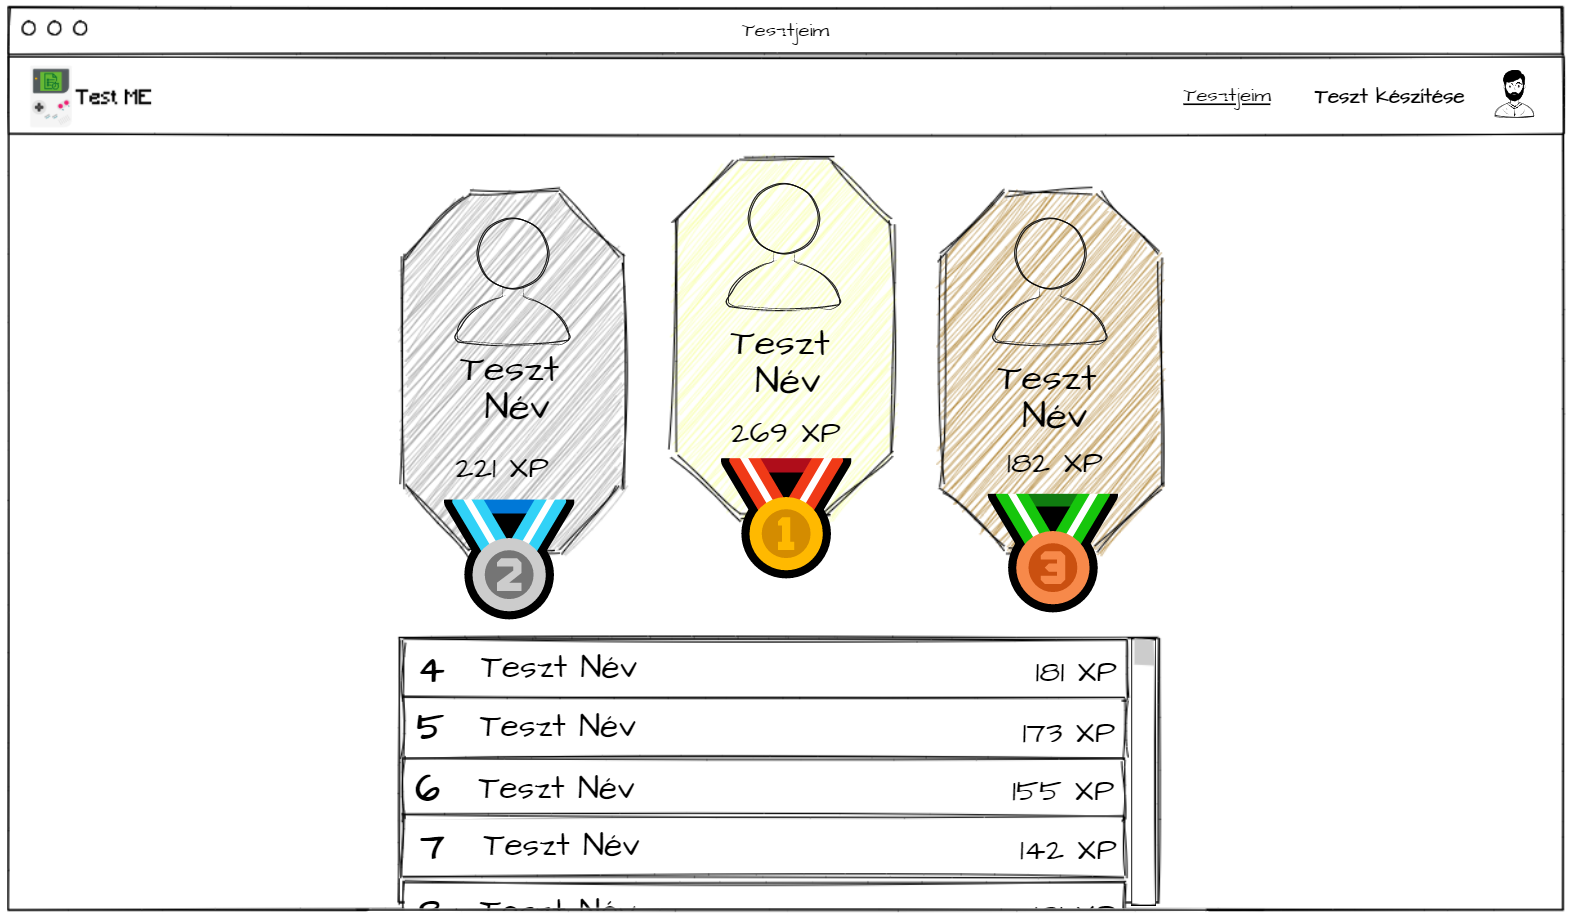
\includegraphics[width=\linewidth]{images/test3_wireframe.png}
    \caption{Teszt eredmény}
    \label{fig:test_finished}
\end{figure}

Miután válaszoltunk minden kérdésre láthatjuk mennyi pontot gyűjtöttünk és hogy kik lettek a legjobbak. \prettyref{fig:test_finished}


\Section{Funkciók}

\begin{itemize}
    \item {Bejelentkezés/Regisztráció}
          \begin{addmargin}[\parindent]{0pt}
              Az oldalon lévő minden funkciót csak regisztráció vagy bejelentkezés után lehet használni. Ez azért fontos hiszen csak így lehet a felhasználónak tesztet küldeni és kitöltés után csak így lehet hozzáadni a profiljához a pontokat és megjeleníteni a nevét a ranglistán. Az weboldal megnyitásakor a felhasználónak be kell jelentkeznie vagy egy helyes e-mail címmel és egy kellően biztonságos jelszóval, regisztrálni kell ha használni szeretné az oldalt.
          \end{addmargin}
    \item {Tesztkészítés}
          \begin{addmargin}[\parindent]{0pt}
              Kahoot!-hoz hasonló teszt készítési felületet szeretnék létrehozni ahol az elkészített teszteket hozzá lehet rendelni diákokhoz és ezután kitölthetik azokat.

              A két következő funkció az egyik legalapvető eleme a játékosításnak, viszont egy jó teszt nélkül értékét vesztik. A fejlődés és a teljesíteni vágyás a belső motiváció számunkra hogy kihívásokat teljesítsünk. Viszont kihívások nélkül a pontok és a jelvények vagy bármi féle jutalmak feleslegesnek tűnnek. Emiatt fontos hogy a tesztek kellő kihívást nyújtsanak hogy aztán a jó eredménnyel járó hasznokat is jutalomnak érezzük.
          \end{addmargin}
    \item {Pontgyűjtés}
          \begin{addmargin}[\parindent]{0pt}
              Minden regisztrált felhasználó rendelkezik majd egy szinttel és egy bizonyos pontszámmal, amelyet a tesztek kitöltésével szerezhetnek.
          \end{addmargin}
    \item {Ranglista}
          \begin{addmargin}[\parindent]{0pt}
              Ranglista a teszt teljes kitöltését követően alakul ki a legtöbbet szerzett pontok alapján.
          \end{addmargin}
    \item {Tesztek diákokhoz rendelése}
          \begin{addmargin}[\parindent]{0pt}
              Teszt létrehozása során email cím vagy valamilyen más egyedi azonosító segítségével hozzá lehetne rendelni diákokhoz a tesztet és így értesülnének róla hogy ki kell tölteniük.
          \end{addmargin}
    \item {Összes hozzárendelt teszt megtekintése}
          \begin{addmargin}[\parindent]{0pt}
              Diákként meg lehet nézni az összes olyan tesztet amit valaki hozzá rendelt a profilhoz. És ezzel együtt a régiek eredményét is, hogy az hogy sikerült mindenkinek.
          \end{addmargin}
\end{itemize}

% TODO: Külön szakaszban érdemes lenne a szerepköröket is részletezni, az azokhoz tartozó jogosultságokat. (Lehet inkább ehhez tartozna inkább a use case diagram.)

% \subsection{Szerepkörök és használati eset}

% Itt látható egy kezdetleges használati eset-modell (use case diagram) ebben benne van a felhasználók információs igényeinek elemzése, funkcionális követelmények elemzése és a modell tartalmazza a rendszerrel szemben támasztott felhasználói követelményeket.
% Látszik hogy kik (esetünkben tanár és diák) és mire akarják használni a rendszert.

% \begin{figure}[h]
%     \centering
%     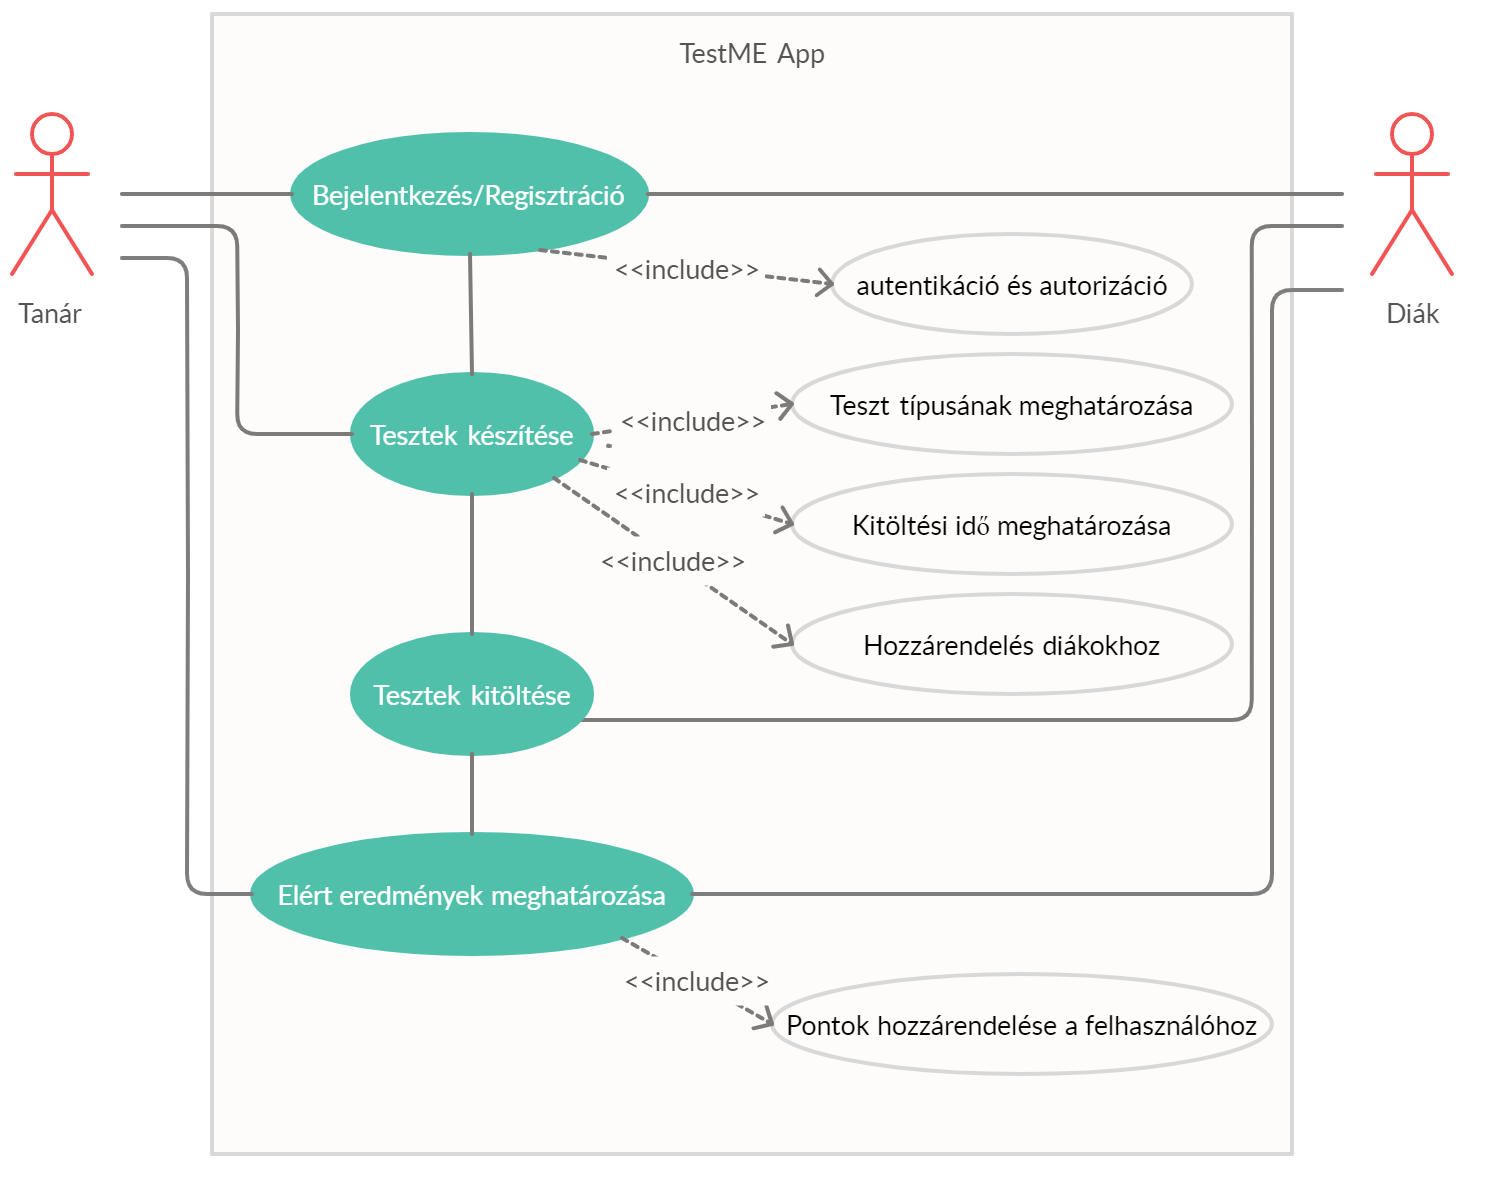
\includegraphics[width=12cm]{images/use_case.png}
%     \caption{Használati eset-modell}
% \end{figure}

% \vspace{5mm}

\Section{Adatmodell}
\label{Adatmodell}

Az adatokat egyed-kapcsolat diagrammon ábrázoltam így a teljes kép könnyebben áttekinthető ezen rendszervázlat alapján.

\begin{figure}[H]
    \centering
    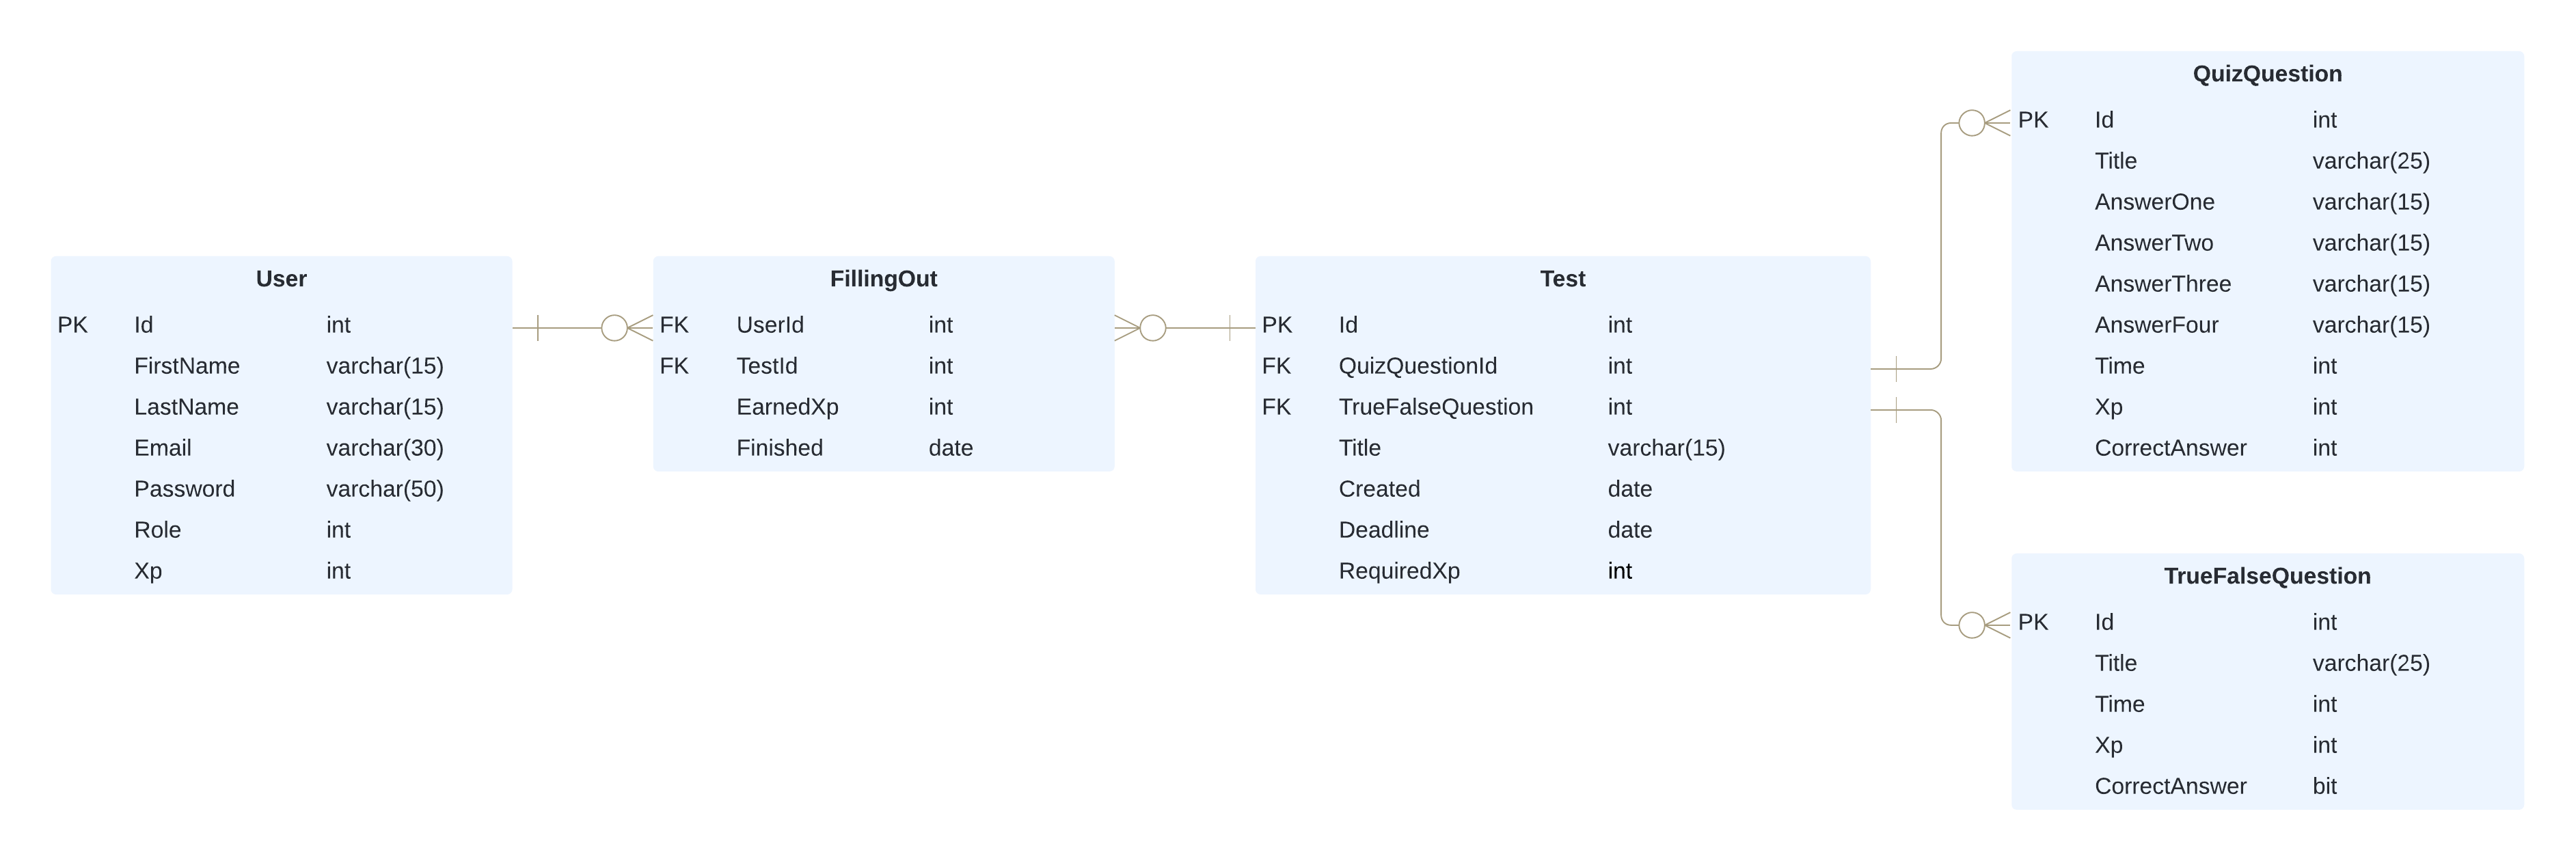
\includegraphics[width=\linewidth]{images/TestME_ER.png}
    \caption{ER modell}
    \label{fig:TestME_ER}
\end{figure}

A diagramm \prettyref{fig:TestME_ER} 5 táblából áll, melyek az alábbiak:
\begin{itemize}
    \item {User}
          \begin{addmargin}[\parindent]{0pt}
              Ez a tábla egy felhasználót reprezentál akinek az alap adatait bekérjük regisztrációkor, ilyen például a keresztnév, vezetéknév, email cím, jelszó. Majd ezen felül még van regisztráció dátuma és hogy visszaigazolta-e az e-mail címét. Valamint meg kell határoznia milyen szerepkörben szeretné használni az oldalt és miután töltött ki tesztet, növekedni fog az xp-je mennyisége így van egy Xp adattag is.
          \end{addmargin}

    \item {Test}
          \begin{addmargin}[\parindent]{0pt}
              A Test tábla egy felhasználó által készített tesztet reprezentál. Egy teszten belül két típusú kérdés lehet az egyik a kvíz a másik az igaz/hamis. Ezenkívül benne van a teszt leírása, a készítő azonosítója, a teszt címe, hogy mikor készült és hogy mi a kitöltési határidő.
          \end{addmargin}

    \item {Question}
          \begin{addmargin}[\parindent]{0pt}
              A Question egy kérdés adatait tárolja amibe beletartozik a kérdés szövege, a négy válasz, az idő, hogy mennyi pontot ér és hogy melyik a helyes válasz.
          \end{addmargin}


    \item {UsersTest}
          \begin{addmargin}[\parindent]{0pt}
              Ez egy kapcsolótáblát képez a Test és a User tábla között. A kapcsolótábla azonosítója a két idegen kulcsból képzett összetett kulcs lesz. Tehát ebbe benne lesz a Test és User tábla idegen kulcsa. Valamint itt tárolódik el hogy felhasználó kitöltötte-e már a tesztet és ha kitöltötte akkor mikor és hogy mennyi pontot ért el. Ez a legtöbbet használt tábla az oldal működése során, hiszen innen szedjük ki az adatokat ha megszeretnénk nézni milyen tesztjeink vannak és ha kitöltjük itt módosítjuk a pontot és a dátumot.
          \end{addmargin}

    \item {Answer}
          \begin{addmargin}[\parindent]{0pt}
              Ez a tábla egy kérdés válaszát tárolja el. Ebben a táblában benne van a kérdés és a UsersTest tábla id-ja, emellett hogy meny idő alatt válaszolt a felhasználó a kérdésre és hogy mi volt a válasza.
          \end{addmargin}

\end{itemize}

\Section{API}

Az alábbi endpointokat szeretném használni az adatok lekérésére és tárolására:
\subsection{Felhasználók}
\begin{itemize}[label={$\bullet$}, topsep=0pt, itemsep=0pt, leftmargin=15pt]
    \item[] {\url{api/users:}}
          \begin{addmargin}[\parindent]{0pt}
              Ezen az endpoint-on tudunk lekérni egy felhasználót bejelentkezéskor, elmenteni a felhasználó session-jét, lekérni a session-t, az id-ját és az email címét. Ezeket mind egy \url{GET} hívással tehetjük meg. Valamint regisztrációkor ide tudjuk elküldeni a felhasználó adatait, a bejelentkezési adatokat és azt hogy ki szeretne jelentkezni egy \url{POST}-tal. Bejelentkezéskor a felhasználó email címét és jelszavát elküldve kikeressük hogy valóban létező, mentett email címet és jelszót küldött el és visszaküldjük a felhasználó adatait.
              \begin{json}
{
    "email": "teszt@teszt.hu",
    "password": "jelszo000"
}
              \end{json}

              Regisztrációkor pedig elküldődnek a felhasználó adatait és bejelentkezteti az oldal. Az elküldött adatok az alábbiak:

              \begin{json}
{
    "roleId": 0,
    "userName": "Levente1999",
    "firstName": "Makszimus",
    "lastName": "Levente",
    "email": "teszt@teszt.hu",
    "password": "Jelszo_.000"
}
              \end{json}

              Valamint lehet egy felhasználó adatait módosítani, \url{PUT} és törölni, \url{DELETE} hívással ugyan azon az endpoint-on: \url{/api/users/{userId}}.
          \end{addmargin}
\end{itemize}

\subsection{Teszt}
\begin{itemize}[label={$\bullet$}, topsep=0pt, itemsep=0pt, leftmargin=15pt]
    \item[] {\url{api/tests:}}
          \begin{addmargin}[\parindent]{0pt}
              Ha a diák ki akarja tölteni a tesztet innen tudjuk lekérni a kérdésekkel együtt. Illetve ha valaki készít egyet akkor ide küldi el az újat.
              Egy elkészített teszt így néz ki ha elküldjük \url{POST}-tal:
              \begin{json}
{
    "description":"Mesterséges intelligencia alapok második zárthelyi dolgozat",
    "userId":"165",
    "title":"Mesterséges intelligencia alapok 2 teszt",
    "created":"2021-01-12",
    "deadline":"2021-01-22",
    "creator":"Makszimus Levente",
    "questions":[
        {
            "problem":"A Turing-teszt teljesítéséért járó arany medál a díj kitűzőjét, Hugh Loebnert ábrázolja?",
            "answerOne":"true",
            "answerTwo":"false",
            "timeLimit":5,
            "xp":3,
            "correctAnswer":0
        }
    ]
}
              \end{json}
          \end{addmargin}
\end{itemize}

\subsubsection{Kérdések}
\begin{itemize}[label={$\bullet$}, topsep=0pt, itemsep=0pt, leftmargin=15pt]
    \item[] {\url{api/tests/answers:}}
          \begin{addmargin}[\parindent]{0pt}
              A kérdést két tábla hivatkozza, az egyik a Teszt mivel egy teszthez tartoznak kérdések. A másik pedig a válasz, azért hogy be tudjuk azonosítani hogy egy válasz melyik kérdéshez érkezett.
              \begin{json}
{
    "problem": "Ha csinálnánk egy csoportos IQ tesztet egy tankör hallgatóival mennyi lenne az átlag?",
    "answerOne": "110",
    "answerTwo": "120",
    "answerThree": "130",
    "answerFour": "140",
    "timeLimit": 10,
    "xp": 5,
    "correctAnswer": 0
}
              \end{json}
          \end{addmargin}
\end{itemize}

\subsubsection{Válaszok}
\begin{itemize}[label={$\bullet$}, topsep=0pt, itemsep=0pt, leftmargin=15pt]
    \item[] {\url{api/answers:}}
          \begin{addmargin}[\parindent]{0pt}
              Itt egy teszt kérdés válasza tárolódik amely kötődik a felhasználói teszthez és magához a kérdéshez.

              \begin{json}
{
    "questionId": 1,
    "usersTestId": 2,
    "responseTime": 5,
    "userAnswer": 4
}
              \end{json}
          \end{addmargin}
\end{itemize}

\subsection{Felhasználó tesztjei}
\begin{itemize}[label={$\bullet$}, topsep=0pt, itemsep=0pt, leftmargin=15pt]
    \item[] {\url{api/users-tests:}}
          \begin{addmargin}[\parindent]{0pt}
              Ha egy diák meg akarja nézni a saját tesztjeit hogy miket kell kitöltenie és miket töltött eddig ki,  akkor azt innen tudjuk lekérdezni. Ezáltal kiírathatjuk őket, azokkal az információkkal hogy befejezték-e már és hogy mennyi pontot kaptak általa. A lekérés a felhasználó id-jának elküldésével történne, és ezt kell visszakapnunk:

              \begin{json}
{
    "id": 1,
    "userId": 1,
    "testId": 1,
    "test": {
        "id": 1,
        "description": "A tesztben csak kvíz kérdések szerepelnek, tehát 4 választási lehetőség közül kell majd választaniuk. Eredményes munkát kívánok!",
        "userId": "152",
        "title": "Mesterséges intelligencia alapok 2 teszt",
        "created": "2021-01-12T00:00:00",
        "deadline": "2021-01-22T00:00:00",
        "questions": [
            {
                "id": 1,
                "problem": "Ha csinálnánk egy csoportos IQ tesztet egy tankör hallgatóival mennyi lenne az átlag?",
                "answerOne": "110",
                "answerTwo": "120",
                "answerThree": "130",
                "answerFour": "140",
                "timeLimit": 10,
                "xp": 5,
                "correctAnswer": 0
            },
            {
                "id": 2,
                "problem": "A Turing-teszt teljesítéséért járó arany medál a díj kitűzőjét, Hugh Loebnert ábrázolja?",
                "answerOne": "true",
                "answerTwo": "false",
                "answerThree": null,
                "answerFour": null,
                "timeLimit": 5,
                "xp": 3,
                "correctAnswer": 0
            }
        ]
},
"finished": "2021-01-13T00:00:00",
"earnedXp": 6
}
              \end{json}

              Valamint amikor egy felhasználó befejezi a tesztkitöltést akkor itt módosításra kerül az xp adattag és megjelenik egy rangsor hogy ki hány pontot ért el. Ehhez le kell kérni az összes játékost akik kitöltötték az a tesztet. Ezt megtehetjük a \url{api/UsersTests/test/testId} endpoint-on. A főoldalon szereplő kitöltött és kitöltetlen tesztek számát is innen tudjuk lekérni.
          \end{addmargin}
\end{itemize}
